\documentclass[11pt]{article}

\usepackage[margin=1in]{geometry}
\usepackage{graphicx}
\usepackage{amsmath,amssymb}
\usepackage{booktabs}
\usepackage{microtype}
\usepackage{natbib}
\usepackage{xcolor}
\usepackage{hyperref}
\hypersetup{colorlinks=true, linkcolor=black, citecolor=blue, urlcolor=blue}

\title{Mapping responses to focal injections of bicuculline along the
rostrocaudal axis of the parafacial lateral region in the adult rat}
\author{}
\date{}

\begin{document}
\maketitle

\begin{abstract}
Active expiration is driven by a conditional oscillator located in the
parafacial lateral (pFL) region on the ventrolateral surface of the medulla,
but the precise rostrocaudal extent and microzonal organisation of this
oscillator have remained unresolved. Prior studies have targeted pFL at
coordinates ranging from $-0.3$ to $+1.0$\,mm relative to the caudal tip
of the facial nucleus (VIIc), reporting heterogeneous combinations of
tonic, late-expiratory, and post-inspiratory abdominal patterns. Here we
systematically compare the response to focal disinhibition of pFL at five
rostrocaudal coordinates within a single experimental preparation.
Bicuculline methochloride (200\,$\mu$M, 200\,nL per side) was bilaterally
pressure-injected at $-0.2$, $+0.1$, $+0.4$, $+0.6$, or $+0.8$\,mm from
VIIc ($n=5$--$7$ per group, total $n=28$) or HEPES vehicle (CTRL, $n=7$)
in anaesthetised, vagotomised adult rats. We recorded abdominal (ABD)
and diaphragm (DIA) electromyograms, airflow, tidal volume,
minute ventilation and oxygen consumption for 20--25\,min and reconstructed
the respiratory cycle as a 3D trajectory. Bicuculline evoked active
expiration at every coordinate, but the magnitude, onset, duration and
metabolic signature of the response followed a clear rostrocaudal
gradient: the most rostral sites ($+0.6$ and $+0.8$\,mm) produced the
fastest onset, the longest-lasting ABD bursts ($17.1$--$17.6$\,min),
the largest peak tidal volume (10.8$\pm$0.5\,ml\,kg$^{-1}$ at $+0.6$\,mm),
and the only drop in $V_{O_2}$ ($-33\%$ and $-25\%$, respectively).
Multivariate trajectory analysis further dissociated the two rostral
sites, with $+0.6$\,mm dominating the inspiratory phase and $+0.8$\,mm
dominating the late-expiratory and post-inspiratory phases. Histology
confirmed that PHOX2B$^+$ retrotrapezoid neurons were not activated by
bicuculline. These results identify a compact rostral core of pFL at
$+0.6$ to $+0.8$\,mm from VIIc, reconcile disparate prior coordinates,
and show that small (\textless$400$\,$\mu$m) shifts along the
rostrocaudal axis qualitatively reorganise the pattern of active
expiration in the adult rat.
\end{abstract}

\section{Introduction}

Breathing is a rhythmic motor behaviour generated by distributed neural
oscillators in the ventral medulla. Inspiration depends on the
preB\"otzinger complex (preB\"otC), a compact cluster of neurons whose
genesis of rhythm has been characterised in detail over three decades
\citep{Smith1991PreBotzinger,Feldman2013Understanding,delNegro2018Breathing}.
Expiration, in contrast, is passive during eupnea but can become active
when metabolic demand rises, airway resistance changes, or central
chemosensory drive increases \citep{Janczewski2006Distinct,Iscoe1998Control}.
Active expiration recruits the internal oblique and transverse abdominal
muscles to drive airflow below the functional residual capacity, and its
loss contributes to ventilatory insufficiency in conditions ranging from
chronic obstructive pulmonary disease to motor neuron disease. A
conditional expiratory oscillator located on the ventrolateral surface of
the medulla, rostral to the preB\"otC and overlapping the caudal aspect of
the facial nucleus, is now widely accepted as the primary substrate of
this active phase
\citep{Pagliardini2011Active,Pisanski2019Parafacial,delNegro2018Breathing}.

This region, the lateral parafacial nucleus (pFL), lies ventral and
lateral to the retrotrapezoid nucleus (RTN), the well-studied
Phox2b-expressing chemosensory nucleus that modulates breathing in
response to central CO$_2$ and pH
\citep{Guyenet2010Central,GuyenetAbbott2013RTN,Takakura2013Phox2b,Marina2010Essential}.
Pharmacological disinhibition of pFL with GABA-A receptor antagonists,
in particular with bicuculline or the mixed GABA-A/glycine antagonist
bicuculline/strychnine, reliably evokes active expiration in anaesthetised
adult rats and in situ preparations, accompanied by phasic
late-expiratory (late-E) bursts in the integrated abdominal electromyogram
\citep{Pagliardini2011Active,Abdala2009Abdominal,Molkov2010Computational,deBritto2017GABAergic}.
Chemogenetic inhibition of pFL neurons, conversely, reduces the intensity
of expiratory muscle recruitment and diminishes but does not abolish active
expiration during sleep in rats
\citep{Huckstepp2015Role,Pisanski2020Parafacial}. The pFL therefore behaves
as a conditional oscillator: permissive for active expiration, but not
obligatory for eupneic breathing.

Despite broad agreement on the functional identity of pFL, its precise
anatomical core has remained surprisingly debated. Different groups have
targeted pFL at rostrocaudal coordinates ranging from $-0.3$ to $+1.0$\,mm
relative to the caudal tip of the facial nucleus (VIIc), the common
anatomical landmark on the ventral medulla
\citep{Pagliardini2011Active,Huckstepp2015Role,deBritto2017GABAergic,Silva2019Importance,Boutin2017Respiratory}.
In juvenile rats, late-expiratory activity and ABD/DIA coupling have been
reported after bicuculline injections at $+0.1$ to $+0.3$\,mm from VIIc
\citep{deBritto2017GABAergic}. In adult rats, chemogenetic and
pharmacological targeting at $+0.5$\,mm produces robust ABD recruitment
\citep{Huckstepp2015Role,Pagliardini2011Active}. A separate line of work,
using bicuculline/strychnine in combination with hypercapnia, localises
the core more rostrally, at $+0.3$ to $+1.0$\,mm from VIIc
\citep{Silva2019Importance}. The qualitative pattern of the ABD response
also varies across these studies: purely tonic expiratory bursts have
been reported with combined GABAergic and glycinergic disinhibition under
CO$_2$, whereas bicuculline alone in normocapnia tends to produce a
mixture of tonic and late-E patterns
\citep{Pagliardini2011Active,deBritto2017GABAergic,Silva2019Importance}.
Whether these differences reflect species, age, coordinate, anaesthetic,
gas composition, or a genuine microzonal architecture of pFL has been
impossible to adjudicate from a meta-analysis of these heterogeneous
studies.

A further question is how active expiration interacts with the rest of
the respiratory cycle when it is driven at different rostrocaudal
coordinates. Active expiration not only recruits abdominal muscles but
also modifies inspiratory timing, inspiratory airflow, post-inspiratory
glottal control, and global minute ventilation through effects on
diaphragm recruitment, upper airway resistance, and sympathetic drive
\citep{Molkov2010Computational,Dutschmann2006Pontine,Zoccal2018Expiratory,Barnett2017Partial,Dhingra2020LateE}.
Most prior studies analyse the ABD response with univariate summaries
(peak amplitude, duration, frequency), which collapse the multi-phase
structure of the respiratory cycle. A multivariate analysis that combines
airflow and the integrated DIA and ABD EMG signals can separate
contributions from late-E, inspiratory, and post-inspiratory windows of
the cycle, and may therefore reveal microzonal differences along the
rostrocaudal axis of pFL.

Here we provide a systematic within-study functional map of pFL in the
anaesthetised, vagotomised adult rat. We bilaterally pressure-injected
bicuculline (200\,$\mu$M, 200\,nL per side) at one of five coordinates
spanning $-0.2$\,mm caudal to $+0.8$\,mm rostral of VIIc, or HEPES
vehicle, and recorded ABD and DIA EMG, airflow, tidal volume, minute
ventilation and oxygen consumption for 20\,min. We verified each injection
site using fluorescent beads and cFos/PHOX2B immunohistochemistry
\citep{Marina2010Essential,Takakura2013Phox2b}. We then quantified the
response with univariate time series and with a multivariate 3D trajectory
of the respiratory cycle. The results show that active expiration is
elicitable at every coordinate tested, but that small shifts along the
rostrocaudal axis ($\leq$\,400\,$\mu$m) qualitatively reorganise the
pattern: the fastest, longest and most metabolically consequential
responses arise at $+0.6$ to $+0.8$\,mm from VIIc, and the $+0.6$ and
$+0.8$\,mm microzones themselves differ in which phase of the cycle they
dominate. These findings reconcile the heterogeneity of prior coordinates
by grounding the expiratory oscillator in a compact rostral core, and
they sharpen the coordinates used by subsequent physiological and
translational studies of active expiration
\citep{Pagliardini2024Parafacial,Jenkin2017Roles,Pisanski2020Parafacial,Pisanski2019Parafacial}.

\section{Results}

We present the results in five parts that each contribute a
complementary layer of evidence for the organisation of pFL along the
rostrocaudal axis. First, we verify the location of the injection sites
and test whether bicuculline engages PHOX2B$^+$ RTN neurons. Second, we
quantify the abdominal (ABD) EMG response at the five coordinates and
establish a rostrocaudal gradient in its reliability, duration, and
onset. Third, we show that the same gradient extends to global
respiratory and metabolic variables. Fourth, we resolve the time course
of the response with bin-by-bin non-parametric comparisons against
vehicle. Fifth, we combine the three physiological signals into a
multivariate 3D trajectory and use it to dissociate two microzones
within the rostral core of pFL.

\subsection{Histological verification of injection sites and local cFos activation}

We first confirmed that bicuculline injections were confined to the pFL
region and did not spread into neighbouring PHOX2B$^+$ chemosensory
neurons of the RTN. Across all 28 bicuculline-injected rats and 7
HEPES-injected controls, fluorescent beads co-injected with the drug
localised the injection cores to one of five rostrocaudal coordinates
($-0.2$\,mm, $n=5$; $+0.1$\,mm, $n=7$; $+0.4$\,mm, $n=5$; $+0.6$\,mm,
$n=6$; $+0.8$\,mm, $n=5$). In CTRL rats injected with HEPES, we observed
an average of $44.7\pm4.0$ cFos$^+$ cells per hemisection along the
rostrocaudal axis of the ventral medulla, of which only $2.3\pm1.0$ were
also PHOX2B$^+$. In bicuculline-injected rats, peak cFos activation
reached $104.5\pm5.1$ cFos$^+$ cells at the core of the injection site,
with local maxima that varied only modestly across coordinates
($-0.2$\,mm $=89.7$; $+0.1$\,mm $=123.1$; $+0.4$\,mm $=110.2$; $+0.6$\,mm
$=98.3$; $+0.8$\,mm $=101.2$). Beyond the injection boundary the count
returned to control levels ($44.8\pm1.2$ cells per hemisection),
consistent with a $\sim$300\,$\mu$m spread of the pharmacological effect.
Critically, the number of double-labelled PHOX2B$^+$/cFos$^+$ cells was
indistinguishable between CTRL ($2.3\pm1.0$) and bicuculline
($2.4\pm0.4$) conditions, indicating that the disinhibition did not
recruit the RTN. Figure~\ref{fig:fig1} summarises these anatomical
controls.

\begin{figure}[ht]
  \centering
  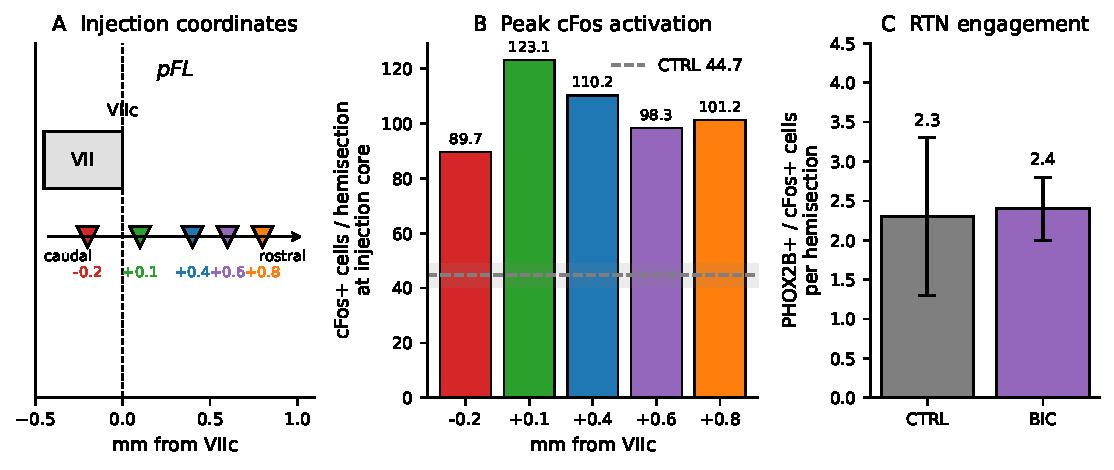
\includegraphics[width=0.95\linewidth]{figures/fig1_schematic_cfos.pdf}
  \caption{\textbf{Experimental design and anatomical verification.}
  \textbf{A} Schematic of the five bilateral rostrocaudal coordinates
  sampled by pressure injection of bicuculline in the parafacial lateral
  (pFL) region. \textbf{B} Peak cFos$^+$ cell counts per hemisection at
  the core of each bicuculline injection (bars) vs.\ the HEPES vehicle
  control (grey dashed line, $44.7\pm4.0$). \textbf{C} Double-labelled
  PHOX2B$^+$/cFos$^+$ cell counts are indistinguishable between CTRL and
  bicuculline conditions, indicating that the retrotrapezoid nucleus is
  not recruited by pFL disinhibition.}
  \label{fig:fig1}
\end{figure}

\subsection{Active expiration is recruited at every rostrocaudal coordinate
but is more robust rostrally}

Bicuculline elicited abdominal (ABD) EMG bursts at all coordinates, but
with a clear rostrocaudal gradient in reliability and in qualitative
pattern. At the most caudal site ($-0.2$\,mm), ABD recruitment was
observed in only 3 of 5 rats, whereas every rat in the four more rostral
groups (n\,=\,5--7) displayed an ABD response. The two most rostral
groups ($+0.6$ and $+0.8$\,mm) showed an additional tonic ABD component
that preceded the late-E peak and was absent in caudal sites. A
post-inspiratory (post-I) ABD peak, a feature diagnostic of glottal-abdominal
coupling, was observed in 5 of 6 rats at $+0.6$\,mm and in no other group.
Quantitatively, the ABD/DIA peak coupling was weak at the caudal site
($-0.2$\,mm $=0.6\pm0.2$) and near unity at more rostral sites
($+0.4$\,mm $=0.96\pm0.02$; $+0.6$\,mm $=0.89\pm0.05$; $+0.8$\,mm
$=0.97\pm0.02$; one-way ANOVA $p=0.015$, $\eta^2=0.43$; Tukey: $-0.2$ vs
$+0.4$\,mm $p=0.024$; $-0.2$ vs $+0.6$\,mm $p=0.048$; $-0.2$ vs
$+0.8$\,mm $p=0.029$). The duration of the ABD response showed an even
stronger gradient: $2.4\pm1.1$\,min at $-0.2$\,mm, compared with
$17.6\pm2.7$\,min at $+0.6$\,mm and $17.1\pm3.3$\,min at $+0.8$\,mm
(one-way ANOVA $p=0.043$, $\eta^2=0.41$). Most strikingly, injections at
$+0.6$\,mm initiated the ABD response on average $88.7\pm32.3$\,s
\emph{before} the second bicuculline bolus, whereas all other groups
began their response 20--40\,s after the second injection (one-way ANOVA
$p=0.041$, $\eta^2=0.57$). Figure~\ref{fig:fig2} summarises these
temporal characteristics.

\begin{figure}[ht]
  \centering
  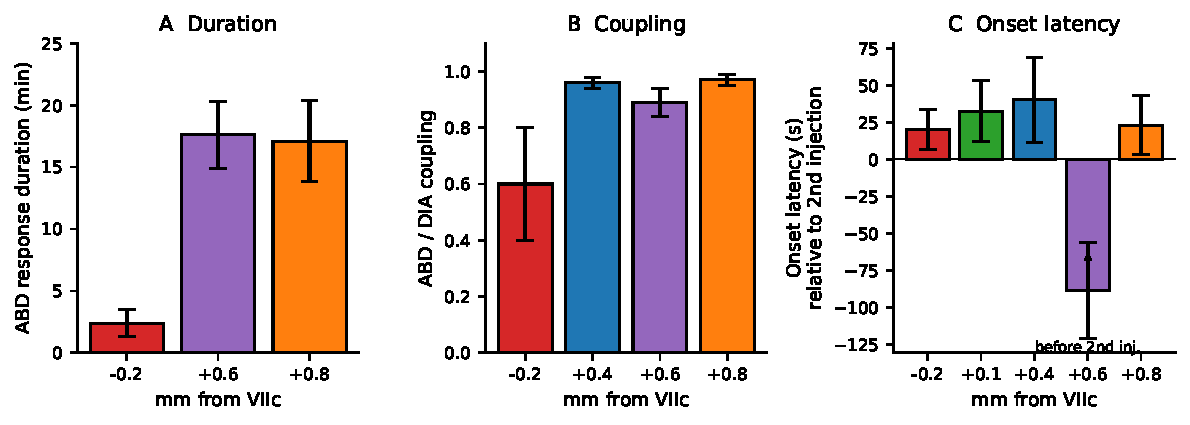
\includegraphics[width=0.95\linewidth]{figures/fig2_abd_temporal.pdf}
  \caption{\textbf{Temporal characteristics of the ABD response to
  bicuculline.} \textbf{A} ABD response duration at the two most rostral
  sites ($+0.6$ and $+0.8$\,mm) greatly exceeds that at the most caudal
  site. \textbf{B} Peak ABD/DIA coupling increases with rostral
  coordinate. \textbf{C} Onset latency relative to the second injection;
  at $+0.6$\,mm the response begins before the second bolus.}
  \label{fig:fig2}
\end{figure}

\subsection{Respiratory frequency, volume and metabolism scale with rostrocaudal
coordinate}

Bicuculline injection caused a drop in respiratory rate at every
coordinate, but the effect reached significance versus baseline only at
the two most caudal sites (one-way repeated-measures ANOVA $p=0.003$,
$\eta^2=0.46$; Bonferroni: $-0.2$\,mm $p=0.03$; $+0.1$\,mm $p=0.005$).
The frequency nadir was reached at 2\,min post-injection at $-0.2$\,mm
($37.08\pm1.36$\,bpm; $-12\%$), at 4\,min for the middle sites
($+0.1$\,mm $=37.2\pm2.0$\,bpm, $-17\%$; $+0.4$\,mm $=40.1\pm1.6$\,bpm,
$-9\%$), and at 6\,min for the two rostral sites ($+0.6$\,mm
$=38.6\pm2.6$\,bpm, $-10\%$; $+0.8$\,mm $=39.1\pm2.2$\,bpm, $-11\%$).
Inspiratory duration shortened in all groups (Ti $=0.279\pm0.034$\,s
vs.\ baseline $0.318\pm0.043$\,s; Wilcoxon rank-sum $Z=3.24$, $p=0.001$),
whereas expiratory duration lengthened (TE $=1.313\pm0.188$\,s vs.\
baseline $1.029\pm0.161$\,s; $Z=4.49$, $p=0.001$), so the caudal slowing
was driven by a prolongation of expiration rather than by a suppression
of inspiration.

Tidal volume (V$_T$) rose in all groups except the most caudal. Peak V$_T$
at $+0.6$\,mm reached $10.8\pm0.5$\,ml\,kg$^{-1}$ (a 29\% increase from
baseline), compared with $7.0\pm0.4$\,ml\,kg$^{-1}$ at $-0.2$\,mm (8\%)
and $8.0\pm0.3$\,ml\,kg$^{-1}$ at $+0.1$\,mm (16\%) (one-way ANOVA
$p=0.01$; Bonferroni $p=0.03$; RM-ANOVA $p=0.01$, $\eta^2=0.44$).
Minute ventilation (V$_E$) decreased by 12\% at $-0.2$\,mm
($255.4\pm16.2$\,ml\,min$^{-1}$\,kg$^{-1}$) but rose by 16\% at
$+0.6$\,mm ($414.3\pm22.7$\,ml\,min$^{-1}$\,kg$^{-1}$) (RM-ANOVA
$p=0.001$, $\eta^2=0.59$). The change in V$_E$ was significantly larger
at the three rostral sites than at $-0.2$\,mm (one-way ANOVA $p=0.001$,
$\eta^2=0.59$; Bonferroni $p=0.0004$). Metabolic O$_2$ consumption
($V_{O_2}$) remained near baseline at the three caudal sites but fell
sharply only at the two rostral sites (+0.6\,mm $=11.8\pm0.8$, $-33\%$;
$+0.8$\,mm $=12.2\pm6.1$, $-25\%$; RM-ANOVA $p=0.0001$, $\eta^2=0.59$;
Bonferroni $p=0.005$). Consequently, the $V_E/V_{O_2}$ ratio rose only
at the two rostral sites, peaking at 6--8\,min post-second injection
($+0.6$\,mm $=34.8\pm3.0$, $+73\%$; $+0.8$\,mm $=38.7\pm12.8$, $+82\%$;
RM-ANOVA $p=0.001$, $\eta^2=0.55$). Figure~\ref{fig:fig3} summarises
these respiratory and metabolic effects. The timing of the respiratory
rate nadir across groups is shown in Figure~\ref{fig:fig5}.

\begin{figure}[ht]
  \centering
  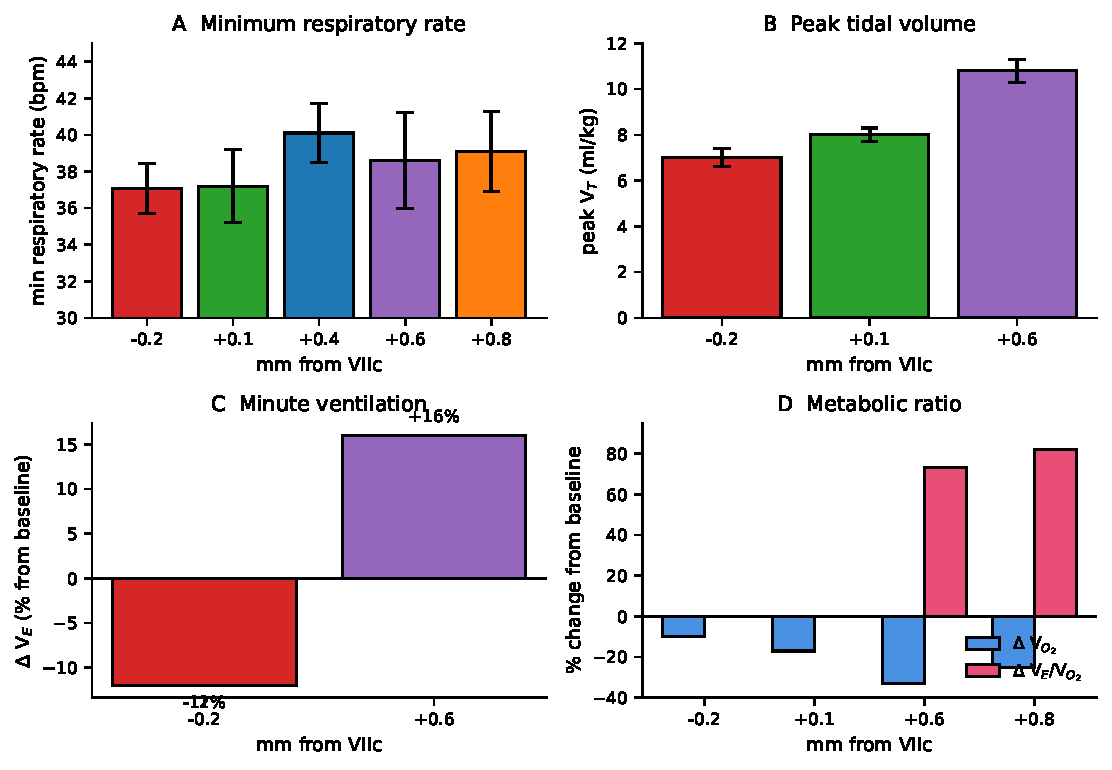
\includegraphics[width=0.95\linewidth]{figures/fig3_respiratory_metabolic.pdf}
  \caption{\textbf{Respiratory and metabolic effects of pFL
  disinhibition.} \textbf{A} Minimum respiratory frequency.
  \textbf{B} Peak tidal volume. \textbf{C} Percent change in V$_E$.
  \textbf{D} Percent change in $V_{O_2}$ (blue) and in $V_E/V_{O_2}$
  (red). The metabolic signature is confined to the two rostral sites.}
  \label{fig:fig3}
\end{figure}

\begin{figure}[ht]
  \centering
  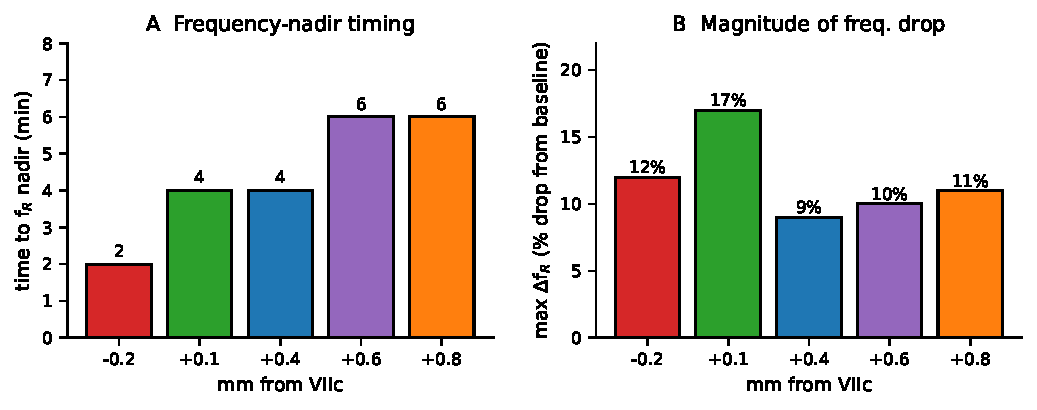
\includegraphics[width=0.85\linewidth]{figures/fig5_nadir_timing.pdf}
  \caption{\textbf{Rostrocaudal gradient in frequency-response timing.}
  \textbf{A} Time from injection to minimum respiratory rate.
  \textbf{B} Magnitude of the frequency drop.}
  \label{fig:fig5}
\end{figure}

\subsection{Time-resolved effects on airflow and the integrated ABD EMG}

To characterise the temporal evolution of the response, we analysed
airflow and the integrated ABD EMG ($\int$ABD) in 2-min bins across the
20-min post-injection window, comparing each bicuculline group against
CTRL and against $-0.2$\,mm using Kruskal--Wallis with Dunn post-hoc
correction. Expiratory airflow at $+0.6$\,mm differed from CTRL from
4\,min (KW $H(5)=14.66$, $p=0.012$; Dunn $p<0.001$) to 12\,min
(KW $H(5)=18.35$, $p=0.003$; Dunn $p<0.001$), and remained more negative
than at $-0.2$\,mm from 8\,min (KW $H(4)=11.41$, $p=0.022$; Dunn
$p<0.001$) to 20\,min (KW $H(4)=10.65$, $p=0.031$; Dunn $p=0.002$). The
$\int$ABD EMG at $+0.6$ and $+0.8$\,mm differed from CTRL and from
$-0.2$\,mm throughout 8--14\,min (KW $H(5)=20.81$, $p<0.001$; Dunn
$p<0.001$), with $+0.8$\,mm still elevated at 16\,min (KW $H(4)=13.56$,
$p=0.009$; Dunn $p=0.002$). On the inspiratory side, airflow at
$+0.6$\,mm was greater than at CTRL from 2\,min (KW $H(4)=13.25$,
$p=0.021$) to 12\,min (KW $H(4)=14.58$, $p=0.012$), and greater than at
$+0.4$\,mm from 10\,min (KW $H(4)=10.50$, $p=0.033$) to 12\,min (KW
$H(5)=10.93$, $p=0.027$). During the post-inspiratory phase, $+0.8$\,mm
produced substantial increases in $\int$ABD activity relative to
$-0.2$\,mm at 6\,min (KW $H(4)=10.37$, $p=0.035$) and 16\,min
(KW $H(4)=9.52$, $p=0.049$). These time-resolved analyses indicate that
the rostral sites dominate not only the magnitude but also the temporal
extent of the abdominal, expiratory, and inspiratory-airflow responses.

\subsection{Multivariate trajectory analysis dissociates the +0.6 and +0.8\,mm
microzones}

To test whether the two rostral microzones drive qualitatively different
deformations of the respiratory cycle, we combined airflow, $\int$DIA,
and $\int$ABD into a 3D trajectory and computed the Euclidean deviation
from baseline during three distinct phase windows: the late-expiratory
``tail'', the inspiratory ``bulb'', and the post-inspiratory ``foot''
\citep{Dutschmann2006Pontine,Dhingra2020LateE}. Compared with CTRL,
bicuculline evoked pronounced late-E tails, inspiratory bulbs, and post-I
feet in all groups, with the notable exception of $-0.2$\,mm, where the
trajectory returned to baseline by 8\,min post-injection. The two rostral
groups elicited the largest late-E deformations; moreover, the $+0.6$\,mm
and $+0.8$\,mm tails peaked at different times. The $+0.6$\,mm tail
exceeded the $-0.2$\,mm tail from 8\,min (KW $H(4)=12.22$, $p=0.016$;
Dunn $p<0.001$) to 12\,min (KW $H(4)=12.34$, $p=0.015$; Dunn $p=0.002$),
whereas the $+0.8$\,mm tail peaked later and remained above $-0.2$\,mm
from 12 to 16\,min (KW $H(4)=10.89$, $p=0.028$; Dunn $p=0.001$). The
inspiratory bulb was largest at $+0.6$\,mm, exceeding that at $-0.2$\,mm
from 8\,min (KW $H(4)=12.59$, $p=0.013$; Dunn $p<0.001$) to 14\,min
(KW $H(4)=10.27$, $p=0.036$; Dunn $p=0.001$). The post-I foot, in
contrast, was largest at $+0.8$\,mm: exceeding that at $-0.2$\,mm from
4\,min (KW $H(4)=10.01$, $p=0.040$; Dunn $p=0.002$) to 16\,min (KW
$H(4)=9.70$, $p=0.046$; Dunn $p=0.001$), with the exception of the 10\,min
and 14\,min bins. Normalising each deformation by its own
trajectory-cloud variability confirmed the same dissociation: $+0.8$\,mm
dominated the late-E and post-I windows through 20\,min, while $+0.6$\,mm
dominated the inspiratory window, peaking at 12\,min (KW $H(4)=10.63$,
$p=0.031$; Dunn $p=0.002$). Figure~\ref{fig:fig4} illustrates these
multivariate deformations.

\begin{figure}[ht]
  \centering
  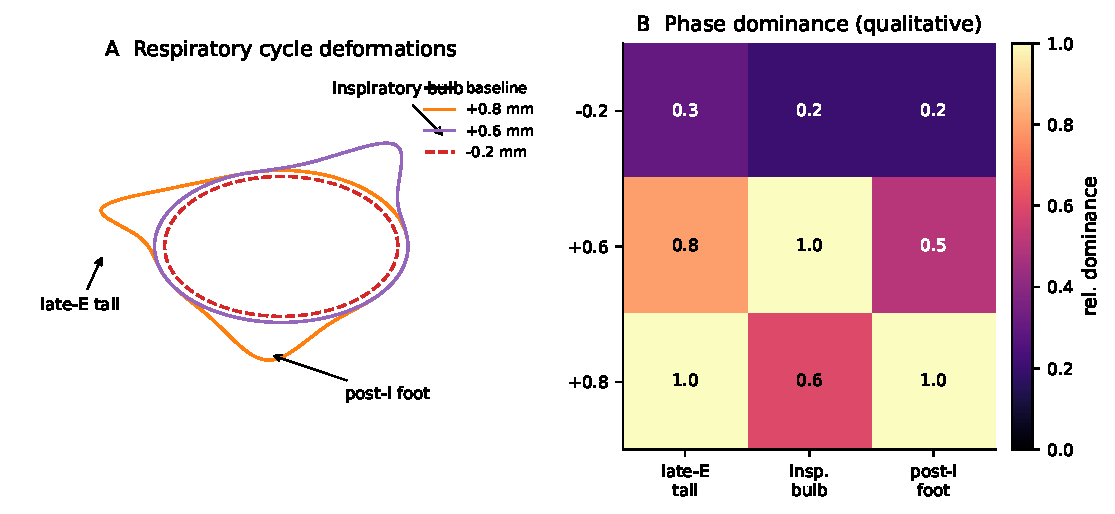
\includegraphics[width=0.95\linewidth]{figures/fig4_3d_trajectory.pdf}
  \caption{\textbf{3D respiratory trajectory dissociates $+0.6$ and
  $+0.8$\,mm responses.} \textbf{A} Schematic cycle in the
  airflow$\times$$\int$DIA$\times$$\int$ABD space, with baseline (black)
  and the qualitative signatures of the three injection sites.
  \textbf{B} Phase-dominance heatmap summarising the statistical
  dissociation of the two rostral microzones.}
  \label{fig:fig4}
\end{figure}

\section{Discussion}

We provide a systematic, within-study functional map of the parafacial
lateral (pFL) region in the anaesthetised, vagotomised adult rat.
Injecting a fixed volume and concentration of bicuculline at five
rostrocaudal coordinates spanning $-0.2$ to $+0.8$\,mm from VIIc, we
find that active expiration is elicitable at every coordinate, but that
the magnitude, temporal extent, phase structure, onset latency, and
metabolic signature of the response follow a clear rostrocaudal
gradient. Five complementary analyses converge on a compact rostral
core of pFL, at $+0.6$ to $+0.8$\,mm rostral of VIIc, that drives the
most robust active-expiratory behaviour.

First, our data locate the functional core of pFL unambiguously to the
rostral half of the tested range. Response duration, ABD/DIA coupling,
onset speed, peak tidal volume and the only rise in $V_E/V_{O_2}$ all
converge on $+0.6$ to $+0.8$\,mm. The $88.7$\,s pre-injection lead at
$+0.6$\,mm is particularly informative: it indicates that a single bolus
already reached threshold for the ABD response, and that a smaller
effective dose is required to activate the oscillator at this coordinate.
This is consistent with the interpretation that the density of
bicuculline-sensitive, expiration-eligible neurons, or the density of
their output synapses on premotor targets, is highest near $+0.6$\,mm.

Second, our multivariate 3D analysis reveals a microzonal organisation
within the rostral core. The $+0.6$\,mm site drives the largest
deformations during the inspiratory phase of the cycle, whereas the
$+0.8$\,mm site drives the largest deformations during the late-E and
post-inspiratory phases. The dissociation is not a quirk of univariate
summaries: in both the absolute 3D distance and the
variability-normalised deformation, $+0.6$\,mm peaks in the inspiratory
bulb while $+0.8$\,mm peaks in the post-I foot and late-E tail. This
separation echoes theoretical
\citep{Molkov2010Computational,Barnett2017Partial} and in-situ
\citep{Abdala2009Abdominal,Dhingra2020LateE} work suggesting that the
expiratory oscillator interacts with the pontine post-I machinery
\citep{Dutschmann2006Pontine} to shape the late-E to post-I transition,
and hints that the pFL may be composed of at least two functionally
distinct microzones whose balance determines the precise pattern of
active expiration.

Third, our within-study comparison reconciles the heterogeneity of prior
coordinates. Previous bicuculline studies have placed the core of pFL at
$+0.1$--$+0.3$\,mm from VIIc in juvenile rats
\citep{deBritto2017GABAergic}, at $+0.5$\,mm in adult rats
\citep{Huckstepp2015Role,Pagliardini2011Active}, and at $+0.3$--$+1.0$\,mm
in adults with combined bicuculline/strychnine and hypercapnia
\citep{Silva2019Importance}. In our dataset the response is graded and
continuous across the full rostrocaudal range rather than confined to a
single point, so each of these prior ranges is consistent with evoking
some fraction of active expiration. The variability in qualitative
pattern---tonic bursts under bicuculline/strychnine with CO$_2$
\citep{Silva2019Importance}; tonic plus late-E patterns under bicuculline
alone in normocapnia
\citep{Pagliardini2011Active,deBritto2017GABAergic}---is compatible with
the microzonal organisation we describe: different coordinate choices,
drug combinations and gas compositions sample different subsets of the
rostrocaudal axis and engage different phase-specific subpopulations.
Our coordinate $+0.6$\,mm, in particular, matches the fastest and largest
ventilatory gain observed in previous studies and is a practical target
for groups that wish to elicit a strong, rapid and prolonged ABD
response in acute preparations.

Fourth, our histological verification clarifies the relationship between
pFL and the RTN. Although pFL lies immediately ventrolateral to the
PHOX2B$^+$ RTN \citep{Guyenet2010Central,GuyenetAbbott2013RTN,Takakura2013Phox2b},
we did not observe any significant increase in cFos$^+$ PHOX2B$^+$
double-labelled neurons after bicuculline, at any coordinate. The
specificity of our pharmacological manipulation therefore lies in pFL
itself, not in the RTN; the effect on breathing is not a secondary
consequence of chemosensory drive. The rostrocaudal effects we report
are therefore attributable to a neuronal population that is distinct
from the PHOX2B$^+$ RTN chemosensors at these coordinates, as previously
suggested by anatomical \citep{Marina2010Essential} and functional
\citep{Huckstepp2015Role,Pisanski2020Parafacial,Jenkin2017Roles} work.

Fifth, our findings have broader physiological and translational
implications. The metabolic consequence of rostral-pFL disinhibition is
notable: at $+0.6$ and $+0.8$\,mm we observed a simultaneous increase in
minute ventilation (up to $+16\%$) and a decrease in O$_2$ consumption
(up to $-33\%$), producing a $+73$--$82\%$ rise in the ventilatory
equivalent for O$_2$. This pattern is not that of a simple metabolic
acceleration; it more closely resembles the ventilatory efficiency of
active exercise \citep{Boutin2017Respiratory,Iscoe1998Control} and the
pattern observed in chronic intermittent hypoxia and sympathetic
overactivity
\citep{Zoccal2018Expiratory,Barnett2017Partial}. The coincident
prolongation of TE, shortening of Ti, rise in V$_T$ and fall in $V_{O_2}$
supports the view that active expiration is not only a motor output but
also a regulatory lever on the cardiopulmonary set-point. In models of
obstructive sleep apnea, motor neuron disease, and ventilatory failure
after brainstem injury, the coordinate-dependent microzonal organisation
we report here is likely to matter: small anatomical shifts during
disease or surgical targeting may produce qualitatively different
respiratory patterns, with different downstream cardiovascular
consequences.

Our study has important limitations. First, the preparation is
anaesthetised and vagotomised; wakeful, intact-vagus behaviour is likely
to differ, particularly in the post-I phase that depends on pontine
gating \citep{Dutschmann2006Pontine,Dhingra2020LateE} and in the
sleep-state-dependent component of active expiration
\citep{Pisanski2020Parafacial}. Second, bicuculline is a relatively
non-specific GABA-A antagonist and does not selectively target a
molecularly defined pFL subpopulation; the apparent microzonal
dissociation at $+0.6$ and $+0.8$\,mm could reflect either a discrete
cell-type difference or a gradient in local circuit connectivity.
Genetically targeted activation, for example using viral expression of
excitatory opsins in candidate expiratory neurons, would provide direct
cell-type evidence. Third, our histological endpoint (cFos) captures
activation over the 60--90\,min window preceding perfusion and cannot
dissociate early from late components of the response. Fourth, we used
adult male Sprague--Dawley rats; sex differences, developmental
differences \citep{deBritto2017GABAergic,Pisanski2019Parafacial}, and
species differences \citep{delNegro2018Breathing} remain to be explored.
Finally, our 3D trajectory analysis summarises an essentially
high-dimensional signal with a small number of phase-specific scalars;
state-space methods that model the continuous dynamics of the cycle
\citep{Molkov2010Computational,Barnett2017Partial,Dhingra2020LateE} will
be useful for future work.

In summary, we provide a high-resolution rostrocaudal map of pFL in the
adult rat. Bicuculline elicits active expiration at every coordinate
between $-0.2$ and $+0.8$\,mm from VIIc, but the magnitude, temporal
extent, metabolic signature and phase structure of the response depend
systematically on the precise rostrocaudal coordinate. The core of the
conditional expiratory oscillator lies at $+0.6$--$+0.8$\,mm, and within
this core the $+0.6$\,mm and $+0.8$\,mm microzones drive qualitatively
different deformations of the respiratory cycle. These results provide a
framework for interpreting the heterogeneity of previous studies, and
they sharpen the anatomical target used by future work on active
expiration in health, exercise, sleep-disordered breathing, and
neurological disease.

\section{Materials and Methods}

\paragraph{Animals.}
Adult Sprague--Dawley rats were used following guidelines of the Canadian
Council of Animal Care under a protocol approved by the Animal Care and
Use Committee of the University of Alberta (AUP\#461).

\paragraph{Surgical preparation.}
Animals were induced with 5\% isoflurane in air and maintained at 1--3\%
isoflurane. A tracheotomy was performed and 30\% supplemental O$_2$ was
delivered throughout the experiment, with expired gases monitored via a
gas analyser (ML 206-1704, ADInstruments). Bilateral vagotomy was
achieved by resecting a 2\,mm portion of the vagus nerve at the
mid-cervical level. Body temperature was maintained at $37\pm1^\circ$C
with a servo-controlled heating pad (55-7022, Harvard Apparatus).

\paragraph{Bicuculline injection.}
Stereotaxic coordinates were set with bregma 5\,mm below lambda, 2.8\,mm
lateral to the midline, and a rostrocaudal coordinate of $-0.2$, $+0.1$,
$+0.4$, $+0.6$, or $+0.8$\,mm relative to the caudal tip of the facial
nucleus (VIIc). A 200\,$\mu$M bicuculline methochloride solution in
HEPES (Sigma-Aldrich; $n=28$) or HEPES/fluorobeads alone (Invitrogen;
CTRL, $n=7$) was bilaterally pressure-injected (200\,nL per side at
100\,nL\,min$^{-1}$) through a 30\,$\mu$m sharp glass pipette. Group
assignments were: $-0.2$\,mm ($n=5$), $+0.1$\,mm ($n=7$), $+0.4$\,mm
($n=5$), $+0.6$\,mm ($n=6$), $+0.8$\,mm ($n=5$), CTRL ($n=7$).

\paragraph{EMG and airflow recording.}
Bipolar fine-wire electrodes were placed in the diaphragm (DIA) and
oblique abdominal (ABD) muscles. Signals were differentially amplified
(AM Systems model 1700, $\times$10\,000 gain) and band-pass filtered
300\,Hz--1\,kHz. Airflow was recorded by whole-body plethysmography, and
tidal volume (V$_T$) was computed by integrating the airflow trace and
scaling with a five-point calibration curve (0.5--5\,ml). All channels
were sampled at 1\,kHz with a 500\,Hz anti-alias filter using a PowerLab
16/30 or 16/35 acquisition system (ADInstruments). Data were analysed in
LabChart7 Pro, Excel 2013, Origin\,9 (OriginLab), and custom MATLAB
scripts (MathWorks). Metabolic O$_2$ consumption ($V_{O_2}$) was derived
from inspired/expired gas concentrations and flow.

\paragraph{Histology.}
Upon completion of recording, rats were transcardially perfused with
0.9\% NaCl followed by 4\% paraformaldehyde in phosphate buffer. Brains
were postfixed, cryoprotected, and sectioned at 30\,$\mu$m on a cryostat
(CM1950, Leica). Serial sections at 120\,$\mu$m spacing, spanning from
400\,$\mu$m caudal to 1000\,$\mu$m rostral to VIIc, were stained for
cFos, PHOX2B, tyrosine hydroxylase and NK1R using overnight primary
antibody incubation in PBS/1\% NDS/0.3\% Triton X-100, followed by
2\,h species-appropriate secondary antibodies (Cy2, Cy3, Cy5 and
rhodamine-red donkey secondaries, Jackson ImmunoResearch), mounting in
Fluorsave (EMD Millipore), and confocal imaging. Fluorobead cores were
used to assign each animal to its rostrocaudal group based on a 3D
distance to VIIc.

\paragraph{Data analysis.}
Baseline and post-injection data were binned in 2-min windows across a
20-min window. Between-group comparisons used one-way ANOVA (Tukey
post-hoc) or one-way repeated-measures ANOVA (Bonferroni post-hoc); when
normality was rejected ($p<0.05$), we used Kruskal--Wallis tests
followed by Dunn post-hoc with the Sidak correction for multiple
comparisons. Paired within-animal comparisons used the Wilcoxon
rank-sum test. Effect sizes are reported as $\eta^2$ (eta squared) from
the ANOVA models. For the 3D trajectory analysis, we constructed per-rat
loops in the airflow $\times$ $\int$DIA $\times$ $\int$ABD space and
computed the Euclidean distance between the injection and baseline
trajectories in three phase windows (late-E, inspiration, post-I). A
variability-normalised version divided each phase-specific distance by
the baseline trajectory spread within the same phase.

\bibliographystyle{plainnat}
\bibliography{references}

\end{document}
